\documentclass[a4paper,11pt]{article}

\usepackage[utf8]{inputenc}

\usepackage{minted}

\usepackage{graphicx}
\usepackage{caption}
\usepackage{subcaption}

\usepackage{pgfplots}
\pgfplotsset{compat=1.18} 

\begin{document}

\title{
    \textbf{My first report}
}
\author{My Name}
\date{Spring Term 2023}

\maketitle

\section*{Introduction}

This is what a report should look like. It is written using the
document class {\tt article} with {\tt a4paper} and {\tt 11pt}
options.  You should of course replace the "My first report" with
something more descriptive and of course have your name below the
title.

What follows is a set of rules and hints on how to write you
reports. Follow these guidelines to make life easier and avoid failing
an assignment by including a screen shot. Do read these guidelines but
also look at the source code of this document. The code will hopefully
show you how to do things. It will also show what packages are
included to get things to work.

\section*{Page layout}

Use vanilla \LaTeX with regular page width and height and single
spaced lines. Don't use any fancy packages that will turn your report
into a Christmas tree, keep it simple!

Since this is a small report you can omit having numbered sections and
you do this by using section commands that end with a {\tt *} (for
example {\tt \textbackslash section* }). You can of course have
subsections etc but if you don't have numbers on the main sections
don't add numbers to the subsections.

\section*{Inserting code}

Code snippets are included using the package {\tt minted}. To get it
to work on you laptop you need to have Pygments installed. If you use
it in Overleaf it should work directly.

\begin{minted}{elixir}
  def append([], b) do b end
  def append([h|t], b) do
    [h | append(t, b)]
  end  
\end{minted}

If you want to include a program statement in running text you can do this
using for example teletype-text: {\tt append([1,2,3],[4,5])}.

The reports that you hand in should be up to four pages long - but not four
pages of code! Use code snippets where you want to describe how things
are done but don't include code just because you have written it. 

\section*{Numbers}

You will include some run-time measurements in your reports. You
should then think about the number of significant figures that you
use. Just because a benchmark took $12345678 \mu s$ does not mean that
you should report it in this way. If you write this in your report
you're implicitly saying - if I do this again the run-time will be the
same. This could be true but I doubt that anything you do on a
computer can be determined with an 8 figure accuracy. The next time
you try it might very well take $12354678 s$. What you report is
maybe $12.3 s$ or $12 s$?

Do read the paragraph above one more time. Handing in a report where
time measurements are reported with more than three figures accuracy is
a sure way to fail - since I then know that you have not read the
above paragraph twice.

\subsection*{Tables}

Numbers are often best presented in a table. You will have to do some
reading on how to format tables but the general structures is quite
easy. This is for example a table with some run-time figures.

\begin{table}[h]
\begin{center}
\begin{tabular}{l|c|c}
\textbf{prgm} & \textbf{run time} & \textbf{ratio}\\
\hline
  dummy      &  115 &     1.0\\
  union      &  535 &     4.6\\
  tailr      &  420 &     3.6\\
\end{tabular}
\caption{Union and friends, list of 50000 elements, run time in micro seconds}
\label{tab:table1}
\end{center}
\end{table}

As you see in the table above, the run time per se might not be
interesting. The interesting thing is how it relates to something
else. Look at the ratios above, it gives you the information that we
are looking for. So when you include numbers, ask yourself why you
have these numbers in the report. What is the purpose, can you
describe it in a better way?

\section*{No f*ing screen shots}

I know that you are all very happy that things actually work and
eagerly want to show what things look like on you screen but please,
don't use {\em screen shots}. It looks ugly and it's impossible to mark or
copy the things that you want to show. It also, most often, show a lot
of irrelevant things so instead of using an image, copy the text and
format it so it's easy to read.

\begin{figure}
  \centering
  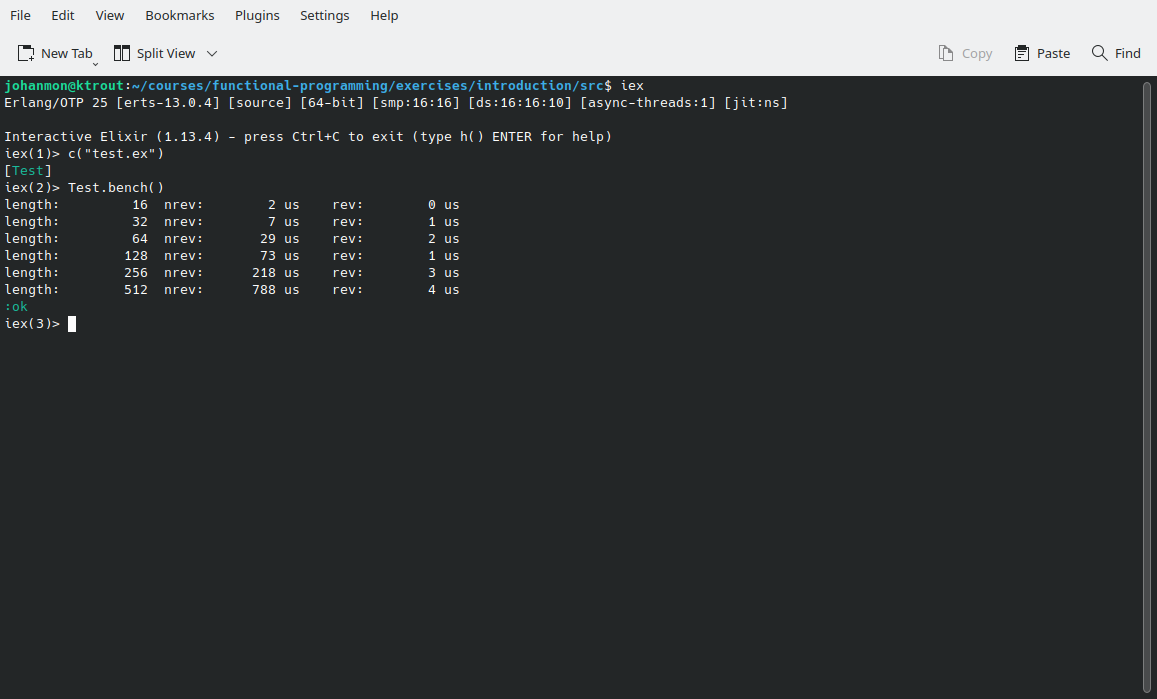
\includegraphics[scale=0.45]{screenshot.png}
  \label{fig:screenshot}
  \caption{This should never be used}
\end{figure}

\section*{Graphs}

Once you start to generate graphs make sure that they are readable and
have sensible information on the axes.

There are many ways to generate graphs but you want to use a way that
minimize manual work. My tool over the years has been {\em Gnuplot}
and if you do not have a favorite tool you could give it a try. The
Gnuplot program is a stand alone program that will generate a
graph that you then can include in you report.

If you work with Gnuplot you should write the commands needed to
generate a diagram in a small script. Take a look in the file {\tt
  fib.p} and you will see how the diagram in Fig.\ref{fig:images} was
created from the data given in {\tt fib.dat} (the {\tt .png} file was
generated from {\tt fib.pdf} using the Linux {\tt convert}
program found in {\tt imagemagick}).

When you include graphs you should make sure that the images you
include are not raster images (gif, png etc) but a vector image that
scales when you zoom-in. In Fig.\ref{fig:images} you see the same
graph saved as a raster image (png) compared to a vector graphic
image. You might not see the difference but if you zoom-in you will
see that the vector image scales.

\begin{figure}[h]
  \centering
  \begin{subfigure}{.5\textwidth}
    \centering
    \includegraphics[scale=0.45]{fib.png}
    \caption{using raster graphics}
  \end{subfigure}%
  \begin{subfigure}{.5\textwidth}
    \centering
    \includegraphics[scale=0.45]{fib.pdf}
    \caption{using vector graphics.}
  \end{subfigure}
  \caption{Difference in image formats.}
  \label{fig:images}
\end{figure}

An alternative to including a graph produced by a separate program is
to describe the graph in \LaTeX. This can be done using the TikZ
library. This library is used to create all types of graphics and the
learning curve is quite steep. The benefit is that the \LaTeX document
becomes self contained and that you are in complete control over the result.

The data can either be written in the latex source file but better read
from a separate file. Reading from a separate file makes it easier to
combine the output from a benchmark with the report. If you construct
your benchmark to produce a file with the x and y values in columns
you can plot them using a simple {\tt \textbackslash addplot}
command. If you do changes to your program you simply run the
benchmark again and re-compile the \LaTeX file.

\begin{figure}
  \centering
  \begin{tikzpicture}
    \begin{axis}[
      xmin=12, xmax=28, ymin=0, ymax=3500,
      xlabel=n, ylabel={time in $\mu s$},
      width=8cm, height=6cm]
      \addlegendentry{run time fib(n)};
      \addplot[] table {fib.dat};
    \end{axis}

  \end{tikzpicture}
  \caption{The same graph using TikZ}
  \label{fig:tikz}
\end{figure}

The graph in Fig.\ref{fig:tikz} is generated using Tikz and as you can
see, I know have the time in "$\mu s$" instead of in "us".

\section*{Errors}

Some \LaTeX errors that I frequently see that could easily be avoided
if you only know where they come from.

\subsection*{less than}

If you in your LaTeX code write "5 \textless\ 7" it will look like 5 <
7 and "9 \textgreater\ 7" will look like 9 > 7. Using the characters
\textless\ and \textgreater\ directly does not work ... so, how did I
do it?  I used the commands {\tt  \textbackslash textless} and {\tt
  \textbackslash textgreater} to generate the symbols \textless\ and
\textgreater.

You could also use {\tt \{\textbackslash tt 5 < 7\}} but then it
will use the teletype font and look like this: {\tt 5 < 7}.

Still another way is to write it using so called {\tt math mode}. This
is a mode used for writing mathematical formulas in a nice way. You
enclose your expression in {\tt \$} signs like this {\tt \$5 < 7\$}
and then it will look like this $5 < 7$.

If you have a larger mathematical expression you enclose it in double
\$ and the result is that it is written centered with some space
around it like this:  $$ 5 < (3 * 8 / 3 ) $$

\subsection*{why strange font}

If you want to write {\em foo} in teletype font you write like this
\verb+{\tt foo}+. If you forget the closing \} then it will look like
this: {\tt foo. Now everything here after until the end of you report
  will look like this. }

\section*{Make}

To automate a process of running benchmarks and compiling a report one
can add everything that needs to be done using a {\tt Makefile}. The
{\tt make} program will determine which files that needs to be
regenerated and re-do only the necessary steps. If you take a look at
the make-file that comes with this report you will see that a change
to the Fibonacci benchmark ({\tt fib.ex}) will trigger the file {\tt
  fib.dat} to be regenerated. This will in turn mean that he diagrams
are regenerated and in the end the \LaTeX report i recompiled.

Working with make-files that causes more than just the report to be
regenerated in one reason why it's more powerful to run \LaTeX on your
own machine rather than using {\em Overleaf}. It does require some
tinkering to get everything to work but once you have it up and running
the development cycle becomes much shorter.





\end{document}
